\documentclass[tikz,border=8pt]{standalone}
% Shared look for every TikZ diagram. Load with % Shared look for every TikZ diagram. Load with % Shared look for every TikZ diagram. Load with \input{../../tools/tikz-style.tex}
\usepackage[T1]{fontenc}
\usepackage{lmodern}
\renewcommand{\sfdefault}{lmr}  % diagrams use the same serif as the text
\usetikzlibrary{arrows.meta, positioning, shapes.geometric, calc, fit, backgrounds}
\definecolor{cblue}{HTML}{4C78A8}
\definecolor{corange}{HTML}{F58518}
\definecolor{cgreen}{HTML}{54A24B}
\definecolor{cred}{HTML}{E45756}
\definecolor{cpurple}{HTML}{B279A2}
\definecolor{cgrey}{HTML}{6B6B6B}
\tikzset{
  every picture/.style={font=\sffamily, line width=1.2pt},
  box/.style={draw=#1, fill=#1!12, rounded corners=4pt, align=center, inner sep=7pt, minimum height=1.1cm},
  box/.default=cgrey,
  arrow/.style={-{Stealth[length=3mm]}, draw=cgrey, line width=1.4pt},
  title/.style={font=\sffamily\bfseries\Large},
  note/.style={font=\sffamily\small, text=cgrey, align=center},
}
\AtBeginDocument{\hyphenpenalty=10000 \exhyphenpenalty=10000}

\usepackage[T1]{fontenc}
\usepackage{lmodern}
\renewcommand{\sfdefault}{lmr}  % diagrams use the same serif as the text
\usetikzlibrary{arrows.meta, positioning, shapes.geometric, calc, fit, backgrounds}
\definecolor{cblue}{HTML}{4C78A8}
\definecolor{corange}{HTML}{F58518}
\definecolor{cgreen}{HTML}{54A24B}
\definecolor{cred}{HTML}{E45756}
\definecolor{cpurple}{HTML}{B279A2}
\definecolor{cgrey}{HTML}{6B6B6B}
\tikzset{
  every picture/.style={font=\sffamily, line width=1.2pt},
  box/.style={draw=#1, fill=#1!12, rounded corners=4pt, align=center, inner sep=7pt, minimum height=1.1cm},
  box/.default=cgrey,
  arrow/.style={-{Stealth[length=3mm]}, draw=cgrey, line width=1.4pt},
  title/.style={font=\sffamily\bfseries\Large},
  note/.style={font=\sffamily\small, text=cgrey, align=center},
}
\AtBeginDocument{\hyphenpenalty=10000 \exhyphenpenalty=10000}

\usepackage[T1]{fontenc}
\usepackage{lmodern}
\renewcommand{\sfdefault}{lmr}  % diagrams use the same serif as the text
\usetikzlibrary{arrows.meta, positioning, shapes.geometric, calc, fit, backgrounds}
\definecolor{cblue}{HTML}{4C78A8}
\definecolor{corange}{HTML}{F58518}
\definecolor{cgreen}{HTML}{54A24B}
\definecolor{cred}{HTML}{E45756}
\definecolor{cpurple}{HTML}{B279A2}
\definecolor{cgrey}{HTML}{6B6B6B}
\tikzset{
  every picture/.style={font=\sffamily, line width=1.2pt},
  box/.style={draw=#1, fill=#1!12, rounded corners=4pt, align=center, inner sep=7pt, minimum height=1.1cm},
  box/.default=cgrey,
  arrow/.style={-{Stealth[length=3mm]}, draw=cgrey, line width=1.4pt},
  title/.style={font=\sffamily\bfseries\Large},
  note/.style={font=\sffamily\small, text=cgrey, align=center},
}
\AtBeginDocument{\hyphenpenalty=10000 \exhyphenpenalty=10000}

\begin{document}
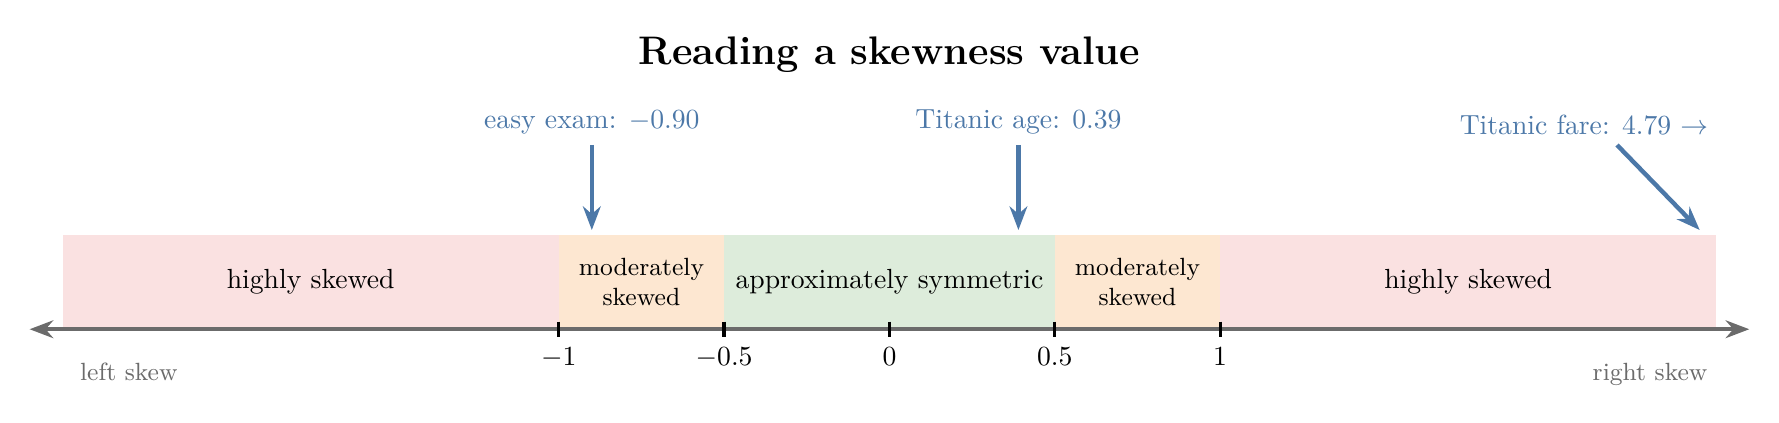
\begin{tikzpicture}[x=4.2cm, y=1.2cm]
  % bands
  \fill[cred!18] (-2.5,0) rectangle (-1,1);
  \fill[corange!20] (-1,0) rectangle (-0.5,1);
  \fill[cgreen!20] (-0.5,0) rectangle (0.5,1);
  \fill[corange!20] (0.5,0) rectangle (1,1);
  \fill[cred!18] (1,0) rectangle (2.5,1);
  \node[align=center] at (-1.75,0.5) {highly skewed};
  \node[align=center, font=\sffamily\small] at (-0.75,0.5) {moderately\\skewed};
  \node[align=center] at (0,0.5) {approximately symmetric};
  \node[align=center, font=\sffamily\small] at (0.75,0.5) {moderately\\skewed};
  \node[align=center] at (1.75,0.5) {highly skewed};
  \draw[arrow, {Stealth[length=3mm]}-{Stealth[length=3mm]}] (-2.6,0) -- (2.6,0);
  \foreach \v in {-1,-0.5,0,0.5,1} \draw (\v,0.08) -- (\v,-0.08) node[below] {$\v$};
  \node[note, below] at (-2.3,-0.25) {left skew};
  \node[note, below] at (2.3,-0.25) {right skew};
  \node[title, above] at (0,2.6) {Reading a skewness value};
  % examples
  \draw[cblue, line width=1.6pt, -{Stealth[length=3mm]}] (0.39,1.95) -- (0.39,1.05);
  \node[cblue, above] at (0.39,1.95) {Titanic age: 0.39};
  \draw[cblue, line width=1.6pt, -{Stealth[length=3mm]}] (2.2,1.95) -- (2.45,1.05);
  \node[cblue, above, align=center] at (2.1,1.95) {Titanic fare: 4.79 $\rightarrow$};
  \draw[cblue, line width=1.6pt, -{Stealth[length=3mm]}] (-0.9,1.95) -- (-0.9,1.05);
  \node[cblue, above] at (-0.9,1.95) {easy exam: $-0.90$};
\end{tikzpicture}
\end{document}
